\documentclass[tikz,border=2pt,11pt]{standalone}
\usetikzlibrary{arrows.meta}
\usetikzlibrary{calc}
\usetikzlibrary{positioning}
\usepackage{amsmath}
\usepackage{amssymb}
\usepackage{tikz}
\begin{document}
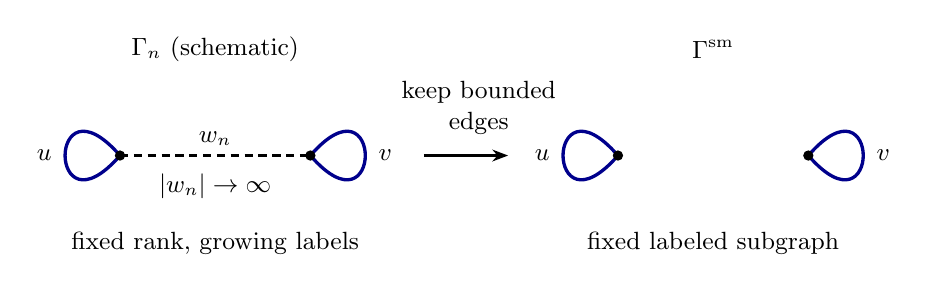
\begin{tikzpicture}[scale=.93, every node/.style={font=\small},
  bounded/.style={draw=blue!55!black,very thick},
  longedge/.style={draw=black,densely dashed,thick}]
\node at (1.3,1.45) {$\Gamma_n$ (schematic)};
\draw[bounded] (0,0) .. controls (-1,1.15) and (-1,-1.15) .. (0,0);
\draw[bounded] (2.6,0) .. controls (3.6,1.15) and (3.6,-1.15) .. (2.6,0);
\draw[longedge] (0,0) -- node[above] {$w_n$}
 node[below=3pt] {$|w_n|\to\infty$} (2.6,0);
\fill (0,0) circle(2pt); \fill (2.6,0) circle(2pt);
\node[left] at (-.8,0) {$u$}; \node[right] at (3.4,0) {$v$};
\draw[-{Stealth[length=2mm]},thick] (4.15,0) -- (5.3,0);
\node[align=center] at (4.9,.65) {keep bounded\\edges};
\node at (8.1,1.45) {$\Gamma^{\mathrm{sm}}$};
\draw[bounded] (6.8,0) .. controls (5.8,1.15) and (5.8,-1.15) .. (6.8,0);
\draw[bounded] (9.4,0) .. controls (10.4,1.15) and (10.4,-1.15) .. (9.4,0);
\fill (6.8,0) circle(2pt); \fill (9.4,0) circle(2pt);
\node[left] at (6,0) {$u$}; \node[right] at (10.2,0) {$v$};
\node at (1.3,-1.2) {fixed rank, growing labels};
\node at (8.1,-1.2) {fixed labeled subgraph};
\end{tikzpicture}
\end{document}
